\chapter{Agrupamento}
Agrupamento é usar as características de entrada para descobrir aglomerações naturais nos dados e para dividir os dados nestes grupos \cite{real2013}. Ou ainda, particionar itens em regiões homogêneas. Um exemplo aplicado a redes sociais é: encontrar comunidades dentro de um grande grupo de pessoas, \citeonline{foundations2012}.

Dentre os algoritmos mais conhecidos de agrupamento estão: K-médias, modelos de mistura gaussianas e clusterização hierárquicas. Um dos métodos mais interessantes para realizar agrupamento é o SOM (Self Organizing Map, Mapa auto-organizável) desenvolvido por Teuvo Kohonen em 1982 \cite{kohonen1982}. Além de realizar o agrupamento com robustez, o SOM é capaz de operar uma redução de dimensionalidade nos dados, dessa forma não somente a morfologia dos agrupamentos é interessante, mas também o mapa gerado pelo algoritmo. Entretanto este algoritmo ainda apresenta o modelo de lote, possuindo fase de treino e uso bem distintas.

\section{SOM}
É possível pensar o algoritmo SOM como uma combinação de dois sistemas menores. Uma parte funciona como uma rede neural competitiva do tipo o vencedor leva tudo. Nesta etapa um dos neurônios da rede é selecionado de acordo com sua semelhança a amostra de entrada, este neurônio é o único vencedor daquela amostra. O segundo sistema acontece depois que o neurônio é escolhido, agora a rede irá se adaptar para incorporar esse novo aprendizado, o peso do neurônio vencedor e de seus vizinhos é alterado, isto é o que dá plasticidade à rede. 
De acordo com Teuvo em, \citeonline{kohonen1982}, o processo auto-organizável do algoritmo pode ser simplificado em quatro etapas:

\begin{enumerate}
\item Um vetor de unidades de processamento que recebem estímulos coerentes de um espaço de eventos e formam funções discriminantes simples com base nas entradas.
\item Um mecanismo que compara as funções discriminantes e seleciona a unidade que possui o maior valor.
\item Algum tipo de interação local, que, simultaneamente, ativa a unidade vencedora e seus vizinhos.
\item Um processo adaptativo que faz os parâmetros das unidades ativadas aumentarem seus valores de função discriminante com base na atual entrada.
\end{enumerate}

Na figura 12 pode-se observar a arquitetura de mapa auto-organizado. As variáveis \textit{epsilon} representam as entradas do sistema, elas são comparadas com todas as unidades de processamento \textit{eta}, e o neurônio que for mais parecido é o vencedor daquela amostra. As unidades de processamento também possuem o conceito de vizinhança, quanto mais próximos uma unidade for da outra, mais parecidas elas serão. A redução de dimensionalidade é alcançada pois, ao fim do treinamento, cada unidade de processamento será um represente do conjunto de entradas que ele foi capaz de selecionar. A figura 13 demonstra a saída de uma rede SOM aplicada a um conjunto de cores, é possível observar que a rede foi capaz de reduzir a dimensionalidade e as características semelhantes ficaram próximas umas das outras.    

\begin{figure}[!h]
\centering
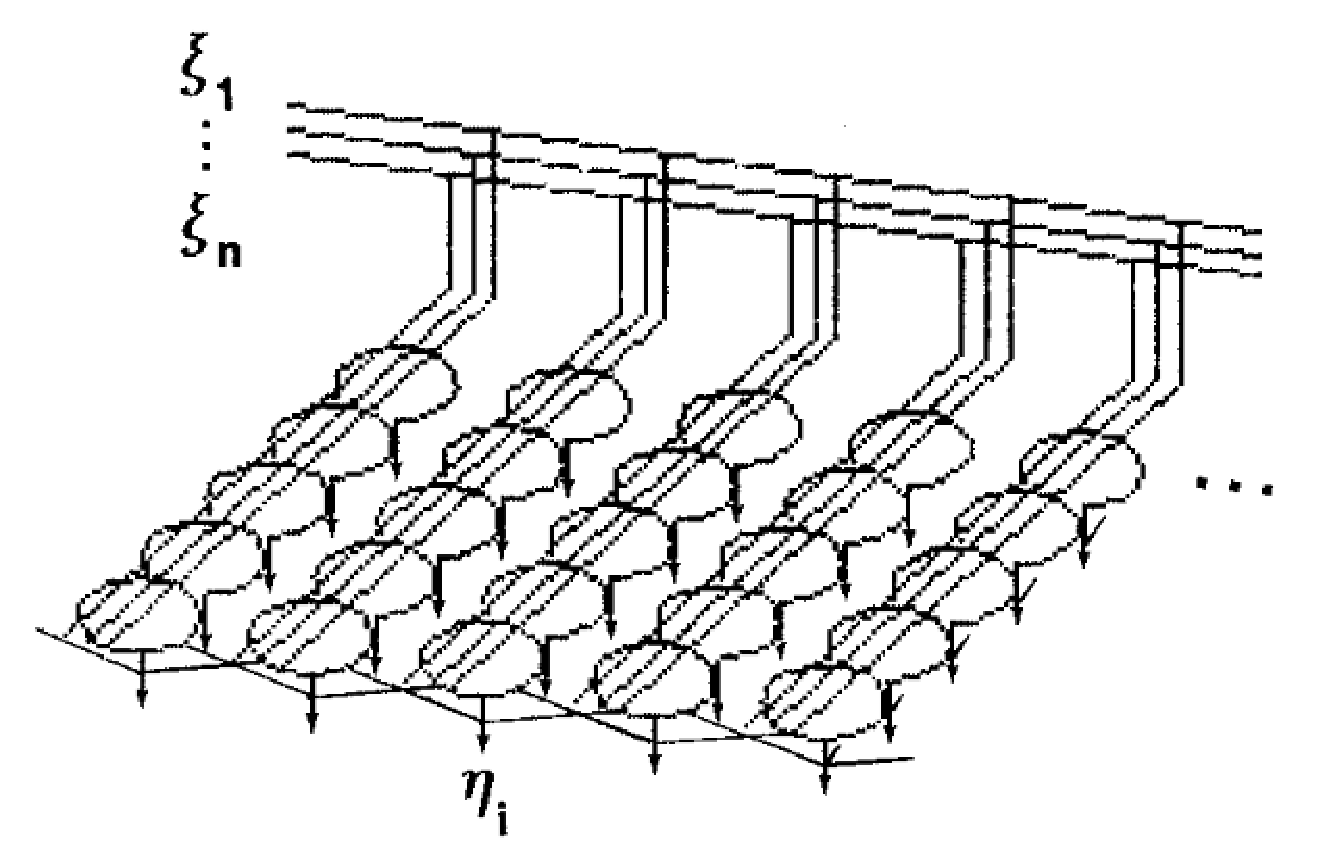
\includegraphics[keepaspectratio=true,scale=0.40]
{figuras/redesom.eps}
\caption{Sistema que Apresenta um Mapa Organizado - \cite{kohonen1982}}
\label{data_titatic}
\end{figure}


\begin{figure}[!h]
\centering
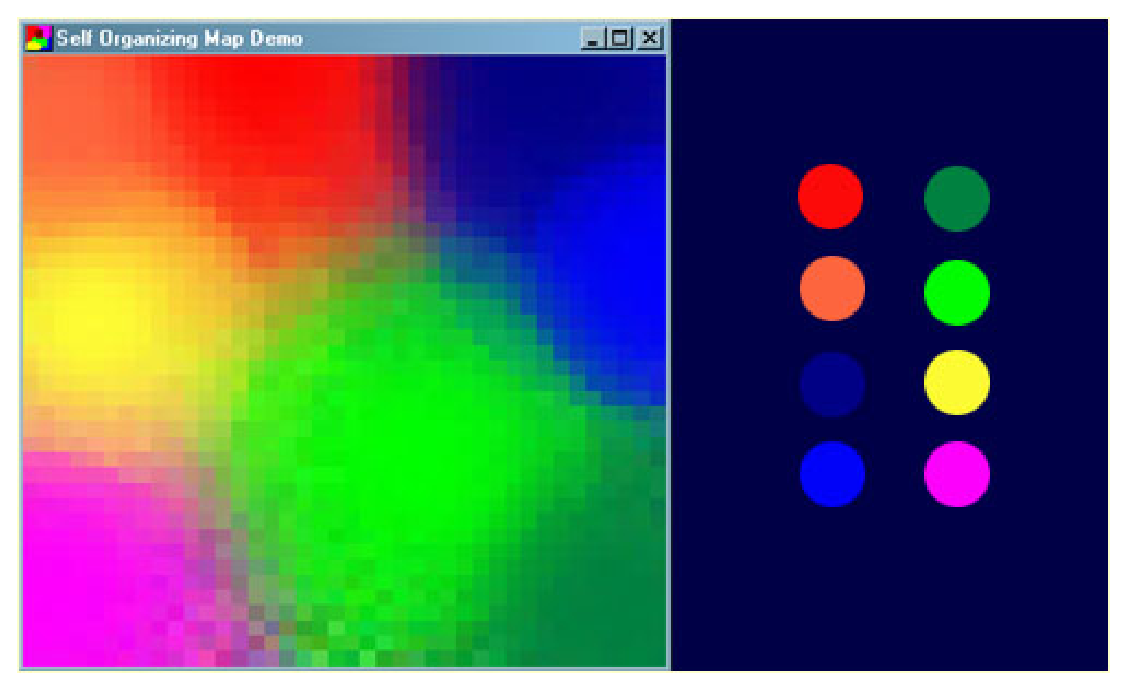
\includegraphics[keepaspectratio=true,scale=0.50]
{figuras/dimensionreduction.eps}
\caption{Exemplo de Redução de Dimensionalidade - \cite{somaijk}}
\label{data_titatic}
\end{figure}

A aplicação SOM pode ser separada em duas etapas, treino e uso. Na etapa de treino as entradas são apresentadas, selecionadas e os parâmetros do mapa são ajustados para incorporar o aprendizado. O processo de treino ocorre até que uma de três condições sejam alcançadas. Ou a quantidade de épocas de treino é atingida, ou o taxa de aprendizado chegue a zero ou a rede atinja algum critério de erro pré-estabelecido que seja aceitável. A etapa de uso é uma variação do treino, as amostras de entrada são apresentadas ao sistema e alguma unidade de processamento será capaz de selecioná-la, a diferença desta etapa para o treino é que não há nenhum aprendizado ou ajuste de parâmetro. O SOM é incapaz de aprender continuamente, pois seus parâmetros internos decaem com tempo, chegando a estabilidade total, onde não há mais aprendizado.

Para compreender cada etapa do algoritmo SOM uma rede bidimensional de neurônios será usada como o mapa auto-organizável. Neste caso cada neurônio possui um conjunto de coordenadas (\textit{x}, \textit{y}) que servem para posicionar os neurônios em um espaço. Em um caso computacional, pode-se pensar nesse mapa como uma matriz quadrada que possui coordenadas (\textit{i}, \textit{j}), \textit{i} para linha e \textit{j} para coluna. O conjunto de pesos de cada neurônio possui a mesma dimensionalidade dos dados de entrada. Abaixo serão descritas as etapas do algoritmo em modo de treinamento.

\subsection{Criação do Mapa e Inicialização dos Pesos} 

A primeira etapa do algoritmo é a criação do mapa. O tamanho da matriz a ser escolhida é uma parametrização do sistema e diferentes tamanhos podem ser úteis para diferentes soluções. Independentemente do tamanho que for escolhido, todos os neurônios da rede irão ajustar seus pesos para representarem as entradas. É necessário então inciar todos os pesos da rede, de acordo com Teuvo em \citeonline{kohonen1982}, uma boa forma de realizar esta etapa é atribuindo pesos randomicamente pequenos a todos os conjuntos de pesos dos neurônios da rede.

\subsection{Escolha do Neurônio Vencedor} 

Para o cálculo do neurônio vencedor, é necessário comparar o dado de entrada com os pesos de cada um dos neurônios do mapa. Aquele neurônio que for mais parecido com a entrada será escolhido como neurônio vencedor. Para realizar esta comparação é necessário estabelecer um método de medir a distância entre a entrada e os neurônios, o neurônio mais parecido será aquele que apresentar menor distância com a entrada. A equação 4.1 mostra a equação de comparação utilizando a distância Euclidiana onde, \textbf{V} representa o vetor de entrada e \textbf{W} é o vetor de pesos do neurônio.

\begin{equation}
    Dist =  \sqrt{\sum_{i=0}^{n} (V - W)^{2}} 
\end{equation}
  
\subsection{Cálculo da Vizinhança}
Depois de cada iteração é necessário atualizar os pesos de cada neurônio que estão dentro do raio de vizinhança do neurônio vencedor. Este raio é um atributo do mapa todo, e é o mesmo para todos os neurônios. De acordo com o número de iterações este raio vai diminuindo, este efeito diminui a plasticidade do mapa de acordo com o tempo, fazendo com o sistema seja capaz de convergir a um estado ideal. A equação de cálculo do raio é definida na equação 4.2 onde, \textit{$\sigma$0} representa a largura inicial do raio que é parametrizado no sistema. \textit{$\lambda$} é uma constante de tempo que determina a velocidade do encolhimento do raio, quanto maior menos o raio diminuirá com o tempo. E \textit{t} é número da atual iteração. 

\begin{equation}
 \sigma (t) =  \sigma_{0} \exp   \big(- \frac{t}{\lambda}\big) \quad \quad t=1,2,3...
\end{equation} 

\subsection{Ajuste dos Pesos}
Todos os neurônios dentro do raio de vizinhança, incluindo o neurônio vencedor, terão seus pesos atualizados para se parecerem mais com a amostra que acabou de ser apresentada. O grau dessa atualização diminui de acordo com a distância entre o neurônio vencedor e seu vizinho, quanto mais distante menor o efeito da atualização. A equação 4.3 torna isso possível onde, \textit{t} representa o número da iteração atual, \textit{L(t)} é o fator de aprendizagem, \textbf{V} representa o vetor de entrada, \textbf{W} é o vetor de pesos do neurônio atual e \textit{$\Theta$(t)} o grau de atualização de acordo com distância do neurônio vencedor. A equação 4.4 mostra os detalhes da equação \textit{L(t)} e a equação 4.5 os detalhes da equação \textit{$\Theta$(t)}. É possível observar que a equação \textit{L(t)} decai exponencialmente um fator de aprendizagem que foi parametrizado inicialmente. Em \textit{$\Theta$(t)}, \textit{\textit{$\sigma$(t)}} é a equação que calcula o tamanho da vizinhança, representada na equação 4.2.


\begin{equation}
W(t + 1) = W(t) +   \theta (t) L(t) (V(t) - W(t))
\end{equation}


\begin{equation}
L(t) =  L_{0} exp  \big( - \frac{t}{ \lambda } \big) \quad \quad t = 1,2,3...
\end{equation}

\begin{equation} 
\theta (t) = exp  \big(- \frac{ dist^{2} }{2  \sigma^{2}(t) } \big)  \quad \quad t= 1,2,3...
\end{equation}

\section{SOM Incremental}
Embora o método SOM seja robusto e amplamente utilizado, ele não possui aplicação em contextos de aprendizagem incremental. O sistema SOM precisa de uma quantidade finita de tempo para receber amostras e absorver as características do espaço de entrada em seu mapa. Em um contexto incremental, não é possível reservar um tempo de treinamento, pois a quantidade de informações que entra no sistema é contínua e as características do espaço de entrada podem mudar com o tempo. Pensando nisso foram desenvolvidos modelos baseados no SOM que apresentam aprendizado incremental.

\subsection{SOM Crescente}
O GSOM (\textit{Growing Self Organizing Map}, Mapa Auto Organizável Crescente), introduz o conceito de um fator de espalhamento. Este fator de espalhamento é responsável por guiar a direção em que o mapa auto organizável cresce. O aprendizado incremental é incorporado neste modelo pelo fato de o mapa poder crescer livremente, no SOM tradicional o mapa tem tamanho fixo. Quando um erro muito alto é alcançado, um novo conjunto de neurônios é criado a partir do neurônio mais parecido que já existe na rede. Outra vantagem do fator de espalhamento é a hierarquização. Através desse fator o mapa é capaz de se sub-espalhar dentro de uma ramificação, significando que o antigo ramo está em uma hierarquia superior ao ramo novo \cite{gsom2000}. A figura 14 mostra o resultado final de um mapa GSOM após ser apresentado a um conjunto de dados com informações sobre os animais de um zoológico.

\begin{figure}[!h]
\centering
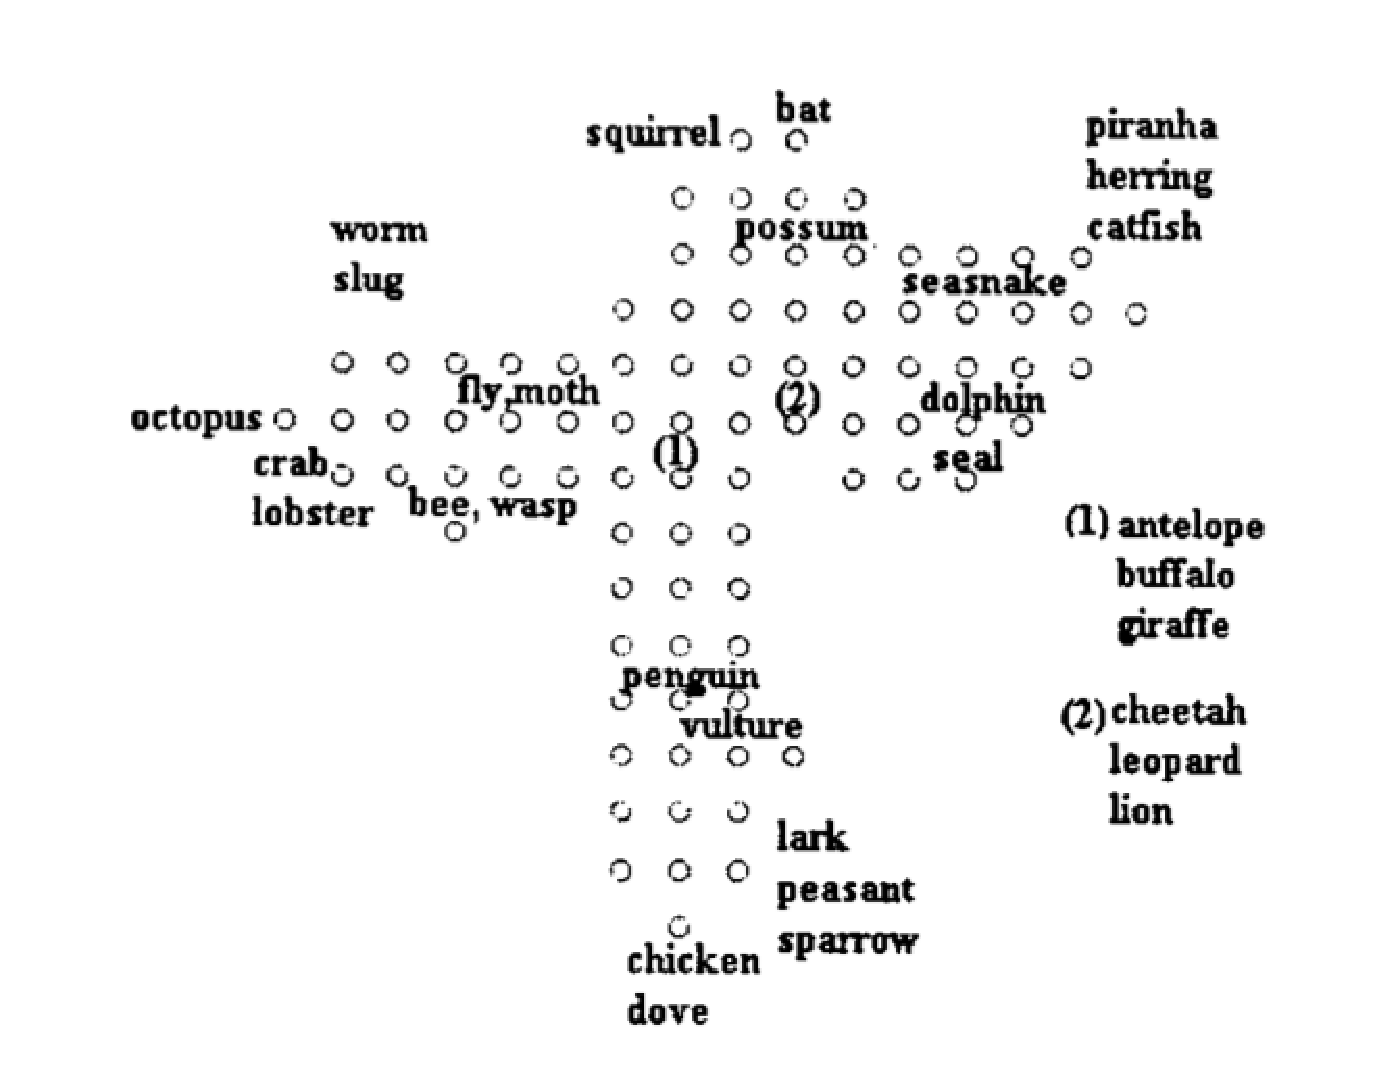
\includegraphics[keepaspectratio=true,scale=0.50]
{figuras/gsom.eps}
\caption{Resultado Final do GSOM - \citeonline{gsom2000}}
\label{data_titatic}
\end{figure}

\subsection{Estruturas Celulares Crescentes}
O Algoritmo de Estruturas Celulares Crescentes é uma variação do SOM que é capaz de automaticamente encontrar uma morfologia e tamanho de mapa. Ao contrário do SOM, que possui seu tamanho e morfologia pré-estabelecidos, este método é capaz de criar e deletar neurônios conforme os conceitos aprendidos pelo sistema. Sua topologia inicial é no formato de um triângulo, que vai crescendo e se adaptando de acordo com os padrões de entrada. É capaz de mesclar várias dimensionalidades na criação dos mapas por ser capaz de criar novos neurônios de maneira empilhada. A figura 15 mostra o resultado final do mapa deste algoritmo, é possível observar que os agrupamentos estão fisicamente separados, pois o sistema foi capaz de deletar os neurônios que estavam no caminho \cite{cellsom2000}.

\begin{figure}[!h]
\centering
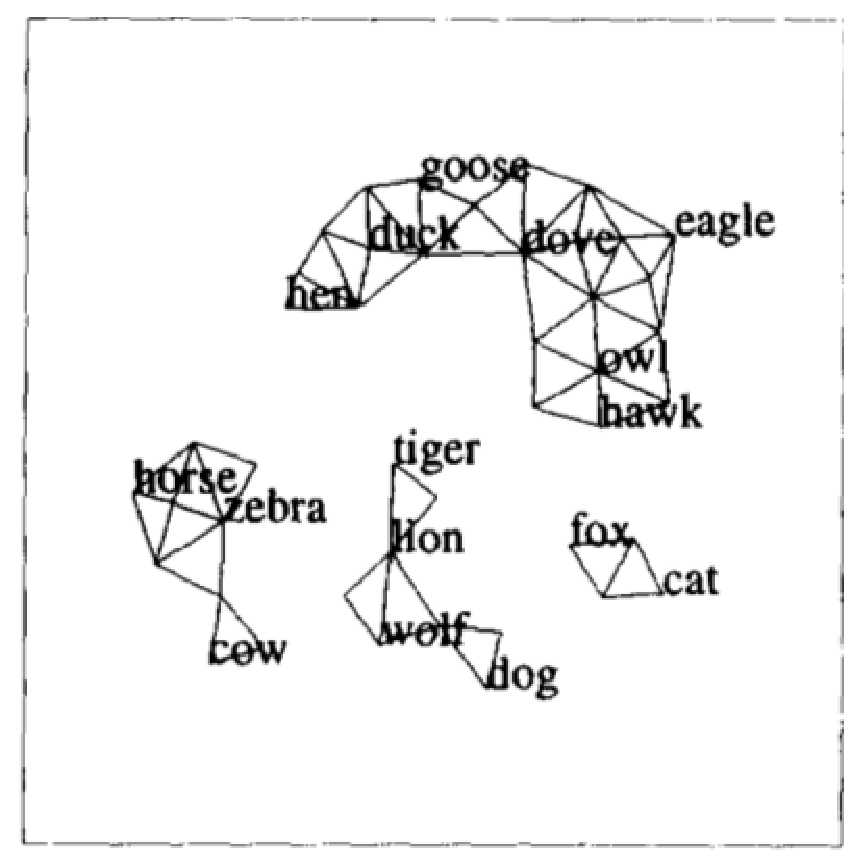
\includegraphics[keepaspectratio=true,scale=0.50]
{figuras/cellsom.eps}
\caption{Mapa do Estruturas Celulares Crescentes - \citeonline{cellsom2000}}
\label{data_titatic}
\end{figure}

\subsection{Mapa Auto Organizável Adaptável com o Tempo}
O TASOM (\textit{Time Adaptative} \textit{Organizing Map} ,Mapa Auto Organizável Adaptável com o Tempo) é o que mais se aproxima do SOM original. A criação do mapa é idêntica, uma morfologia e tamanho devem ser definidas antes do começo do uso da rede. A rede SOM possui uma taxa de aprendizado e raio de vizinhança que são universais para todos os neurônios da rede. Além dessa universalidade, o aprendizado e a vizinhança no SOM são dependentes do tempo. O TASOM introduz o conceito de que cada neurônio possui seu própio raio de vizinhança e taxa de aprendizado. 

No TASOM a taxa de aprendizado de cada neurônio é determinada por uma função de distância entre o vetor de entrada e os pesos do neurônio. O raio de vizinhança é dependente da distância entre os pesos do neurônio com os pesos de seus vizinhos. Estas duas características tornam o TASOM livre da variável de iteração, portanto ele não necessita de um período de treinamento e é capaz de se ajustar conforme a precisão de seus agrupamentos e da coesão entre um neurônio e seus vizinhos. Este algoritmo é capaz de aprender novos conceitos não por criar ou deletar novos neurônios, mas por esquecer informações antes aprendidas e dar um novo aprendizado para os neurônios \cite{tasom2001}.

O TASOM é o método SOM incremental mais simples em seu conceito dos que aqui foram apresentados, além de criar um mapa idêntico ao do SOM tradicional. Por ser capaz de criar um mapa equivalente ao do SOM clássico é possível comparar o desempenho dos dois algoritmos em um ambiente não incremental. Por estes motivos o algoritmo TASOM foi escolhido como objeto de estudo de um método não supervisionado de agrupamento incremental.  



 

 










